\documentclass[12pt]{article}
\usepackage[letterpaper, top=1.25in, bottom=1.25in, left=1in, right=1in]{geometry}
\usepackage{fancyhdr} % http://ctan.org/pkg/fancyhdr
\usepackage{hyperref}
% \usepackage{xcolor}
\usepackage{graphicx}
\usepackage{indentfirst}
\usepackage[export]{adjustbox}

% % % % % % % % % % % % 
% Citation formatting %
% % % % % % % % % % % % 

\usepackage[style=ieee]{biblatex}
\addbibresource{sources.bib}

% % % % % % % % %
% Hyperlinking  %
% % % % % % % % %

\hypersetup{
    colorlinks=false, % set true if you want colored links
    linktoc=all,     % set to all if you want both sections and subsections linked
    % linkcolor=black,  %c hoose some color if you want links to stand out
    % citecolor=black
    % urlcolor=black
}

% % % % % % % % % % % % % % % %
% Global title, author, date  %
% % % % % % % % % % % % % % % %

\title{Exploring Smart Sensor Systems}
\author{Nathan Quadras \& Kosta Sergakis}
% \author1{Quadras \& Sergakis}
% \date{\today}
\date{April 28, 2025}
\makeatletter
\let\runauthor\@author
\let\runtitle\@title
\let\rundate\@date
\makeatother

% % % % % % % % % % %
% Header and Footer %
% % % % % % % % % % %

\pagestyle{fancy} % change page style to fancy
\fancyhf{} % clear header/footer
\setlength{\headheight}{15pt}
\fancyhead[L]{Quadras \& Sergakis}
\fancyhead[C]{\runtitle}
\fancyhead[R]{\rundate}
\fancyfoot[C]{\thepage} % \fancyfoot[R]{\thepage}
\renewcommand{\headrulewidth}{0.4pt} % default \headrulewidth is 0.4pt
\renewcommand{\footrulewidth}{0.4pt} % default \footrulewidth is 0pt

% \usepackage{natbib}
\begin{document}

    % % % % % % % %
    % Title Page  %
    % % % % % % % %
    
    \begin{titlepage}
        \begin{center}
            \vspace*{1.5cm}
            
            \textbf{\runtitle}
            
            \vspace{1cm}
            
            An exploration of:\\
            \vspace{0.25cm}
            Slip Angle Sensors
                
            \vspace{1cm}
            
            \textbf{\runauthor}
            
            \vfill  
            
            \vspace{1cm}

            
\includegraphics[width=0.3\textwidth]{resources/michigan-state-logo-png-transparent.png}
                
            Electrical and Computer Engineering\\
            Michigan State University\\
            East Lansing, Michigan\\
            \rundate
                
        \end{center}
    
    \end{titlepage}


    % % % % % % % % % % %
    % Table of Contents %
    % % % % % % % % % % %

    \setcounter{secnumdepth}{0} % removes section numbers
    % \maketitle
    
    \tableofcontents
    
    \newpage

    \section{Introduction}
        
    Vehicles are more attainable than ever and are advancing quickly. Modern cars 
    are equipped with sophisticated systems that enhance performance, safety, and driver 
    comfort. Vehicle dynamics is a tremendous topic and an area of growing interest, especially 
    as more automated driving technologies emerge. Vehicle dynamics is the study of vehicle 
    motion in relevant user operations \autocite{Jacobson_2016}, which encompasses factors like kinematics, forces, 
    and moments acting on a vehicle during acceleration, braking and steering. The core of vehicle 
    dynamics involves the following primary aspects: the mechanisms that disturb a vehicle’s state 
    (inputs) and the mechanisms through which the vehicle responds (outputs). Arguably the most 
    critical aspect of vehicle dynamics is tire behavior, specifically how a tire generates lateral 
    force during cornering. Central to this behavior is the concept of slip angle – the difference 
    between the direction a vehicle is traveling and the direction that the body of the vehicle is 
    pointing (heading vs. true heading) \autocite{Racelogic_2015}. Understanding slip angle is essential for analyzing 
    handling characteristics, improving stability control systems, and optimizing driver feedback.
        
        \subsection{Vehicle Dynamics}

        Performance driving, autonomous driving and commuter driving all require the same characteristic: 
        control. Controllable vehicles are what makes rapid maneuvers possible. On the other hand, the required 
        motion must be stable to maintain directional stability under disturbances \autocite{MMM}. 

        \begin{center}
            \vspace{0.5cm}

            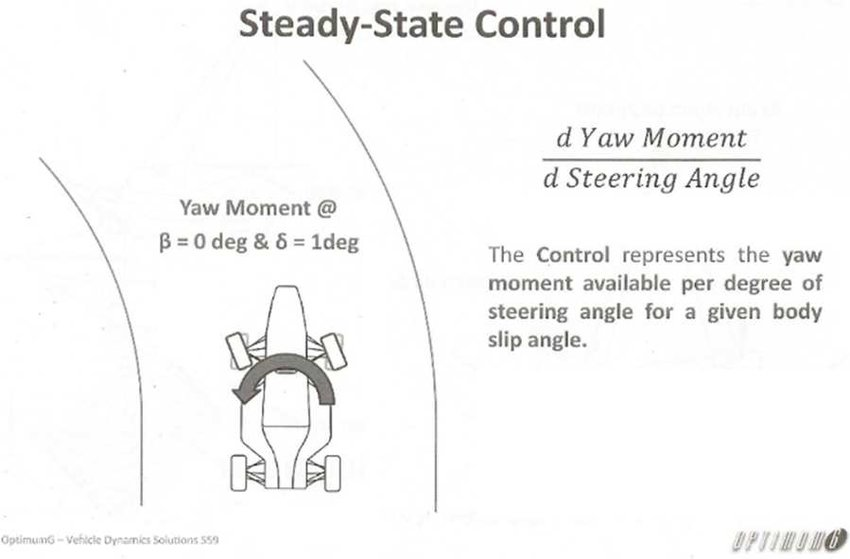
\includegraphics[width=0.7\textwidth]{resources/Defining-of-control-Claude-Rouelle-Applied-VD-seminar.png}

            \vspace{0.5cm}

            \textbf{Figure 1: Definition of Control} \autocite{MMM}
            \label{control}
        
        \end{center}

        \begin{center}
            \vspace{0.5cm}

            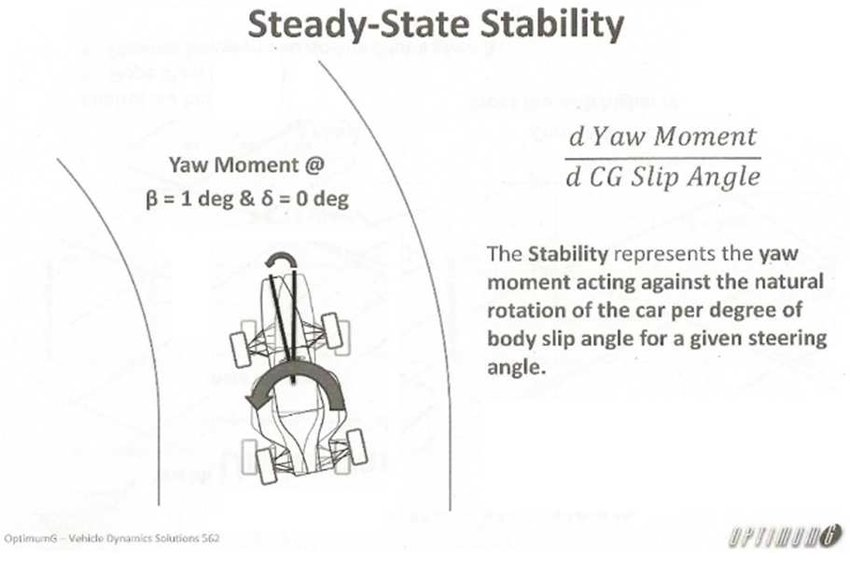
\includegraphics[width=0.7\textwidth]{resources/Defining-of-stability-Claude-Rouelle-Applied-VD-seminar.png}

            \vspace{0.5cm}

            \textbf{Figure 2: Definition of Stability} \autocite{MMM}
            \label{stability}
        
        \end{center}

        It is crucial to define the tractive limit of the vehicle, or the “safety margin” to determine the range of 
        possible motions that the vehicle can produce while maintaining stability \autocite{MMM}. Slip angle is incredibly important 
        because it enables the concepts mentioned above. In other words, slip angle determines vehicle maneuverability. If 
        slip angle is observed, various states of the vehicle can be determined. 

        % \begin{center}
        %     \vspace{0.5cm}

        %     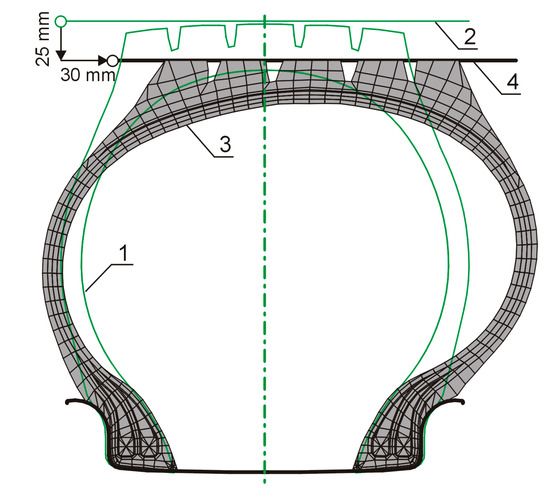
\includegraphics[width=0.5\textwidth]{resources/applsci-10-04326-g009-550.jpg}

        %     \vspace{0.5cm}

        %     \textbf{Figure 3: Tire Deformation} \autocite{app10124326}
        %     \label{tire_deformation_1}
        
        % \end{center}

        \begin{center}
            \vspace{0.5cm}

            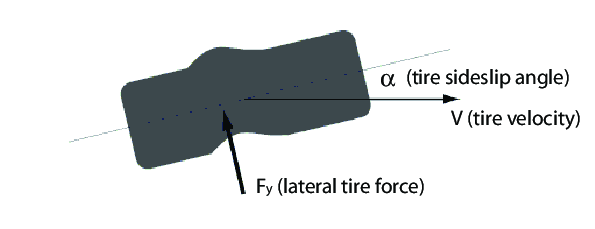
\includegraphics[width=0.8\textwidth]{resources/Lateral-tire-deformation.png}

            \vspace{0.5cm}

            \textbf{Figure 3: Tire Deformation} \autocite{inproceedings}
            \label{tire_deformation_2}
        
        \end{center}

        \begin{center}
            \vspace{0.5cm}

            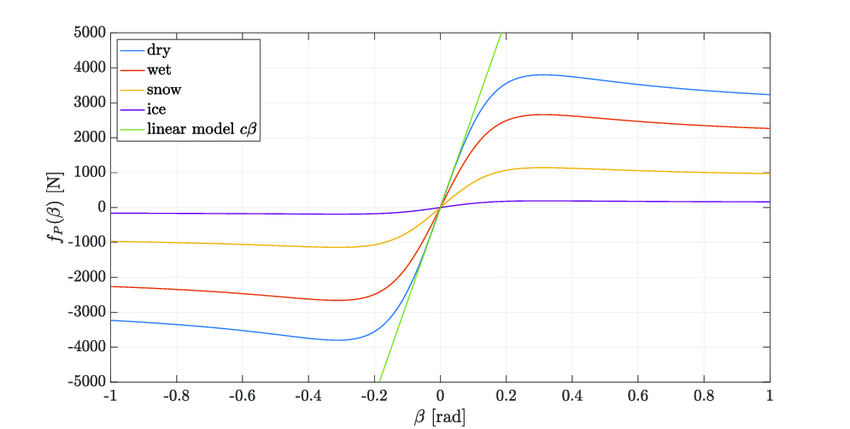
\includegraphics[width=1\textwidth]{resources/Pacejkas-tire-model.png}

            \vspace{0.5cm}

            \textbf{Figure 4: Example Pacejka Tire Model} \autocite{pacejka}
            \label{pjka}
        
        \end{center}

        \begin{center}
            \vspace{0.5cm}

            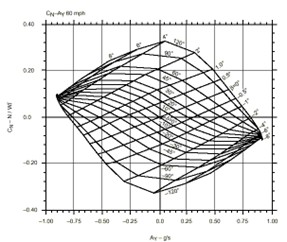
\includegraphics[width=0.5\textwidth]{resources/tn_MMM807.jpg}

            \vspace{0.5cm}

            \textbf{Figure 5: MMM} \autocite{Milliken_Research_Associates}
            \label{MMMa}
        
        \end{center}

        A common way to observe/determine the limits of a vehicle is through a Yaw Moment Diagram, or the MRA Moment Method 
        (MMM) \hyperref[MMMa]{[Figure 5]} \autocite{Milliken_Research_Associates}. A critical component of the Yaw Moment Diagram would be the quantification of the forces necessary to hold 
        a vehicle through a turn. As shown in  \hyperref[tire_deformation_2]{Figure 3}, a primitive to determining the lateral force of a tire is the slip angle. 
        Pacejka’s formula can display the relationship between slip angle and lateral tire force as shown in \hyperref[pjka]{Figure 4}. Ultimately, 
        the goal is to determine the limits of the vehicle to prevent drivers from reaching the point of no return; a loss of 
        stability, leading to control being removed from the driver.

        \subsection{Overview \& Motivation}
        
        This smart system focuses on real-time slip angle estimation and control for ground vehicles. Accurate knowledge of 
        slip angle enables Advanced Drive-Assistance Systems (ADAS), traction control, and autonomous driving algorithms to make 
        more informed decisions when navigating corners, avoiding obstacles, or maintaining control on low-friction surfaces. 
        
        The motivation for this system stems from the growing demand for safer and more responsive vehicles in both human-driven 
        and autonomous applications. While modern vehicles are equipped with various sensors, slip angle is notoriously expensive 
        to measure directly due to the niche, specialized equipment involved. By designing a smart system capable of observing slip 
        angle in real-time using accessible components, this solution offers a cost-effective and scalable method to improve vehicle 
        safety, performance, and driver confidence across a wide range of driving conditions. 

    \section{System Level Design}
        
        \begin{center}
            \vspace{0.5cm}

            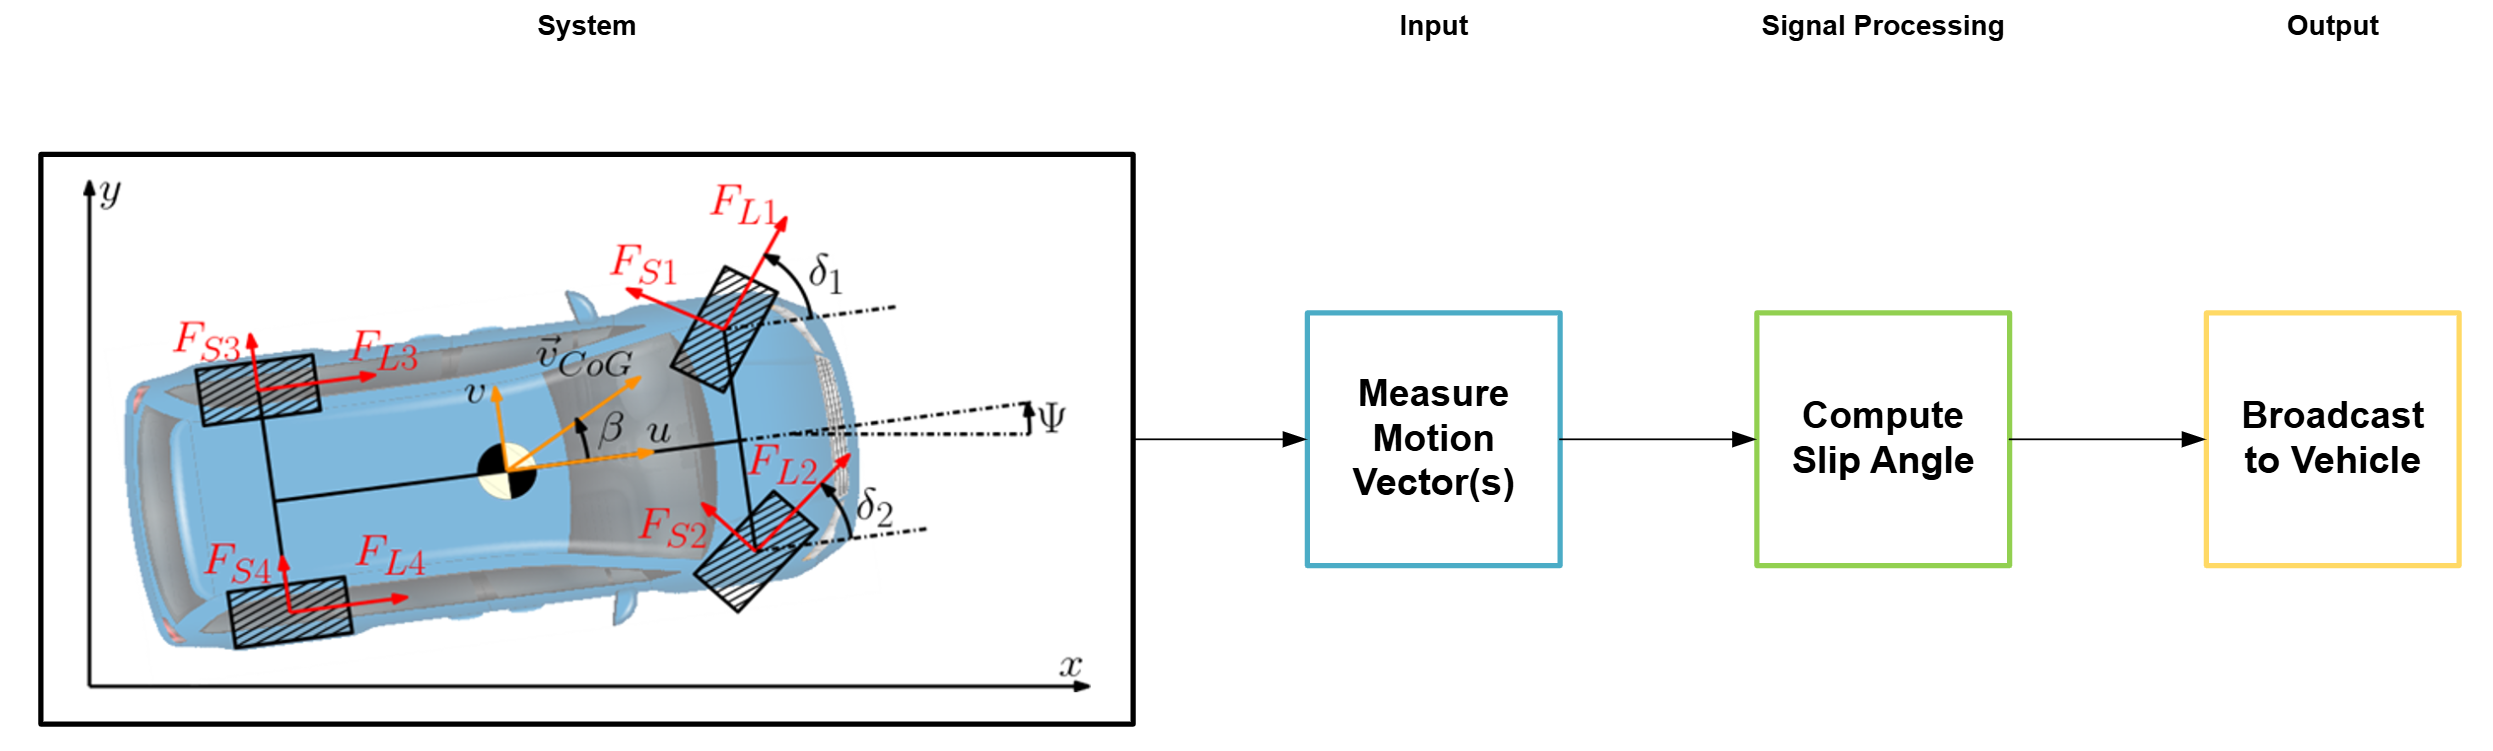
\includegraphics[width=1\textwidth]{resources/image.png}

            \vspace{0.5cm}

            \textbf{Figure 6: System Diagram}
            \label{diag}
        
        \end{center}
        
        First, an optical sensor would be required to detect ground-relative lateral and longitudinal displacement by tracking the surface motion 
        beneath the tire. Next, the vehicle’s heading direction would need to be determined through drift-compensated orientation data, for reliable 
        direction estimation over time. Additionally, a simple system status indicator would be required to provide immediate visual feedback on operational 
        states including normal function, error detection, and idle shutdown. A high-performance microcontroller would constitute the brain of this device 
        and would be responsible for acquiring sensor data, computing the instantaneous slip angle by comparing ground motion to heading, and transmitting 
        the results to external systems over a reliable communication interface, all with minimal latency. Finally, components necessary for communication 
        with the vehicle’s internal network must also be incorporated. Together, these elements operate in a coordinated real-time loop, enabling direct, 
        ground-referenced slip angle estimation critical for dynamic vehicle behavior analysis.

        \begin{center}
            \vspace{0.5cm}

            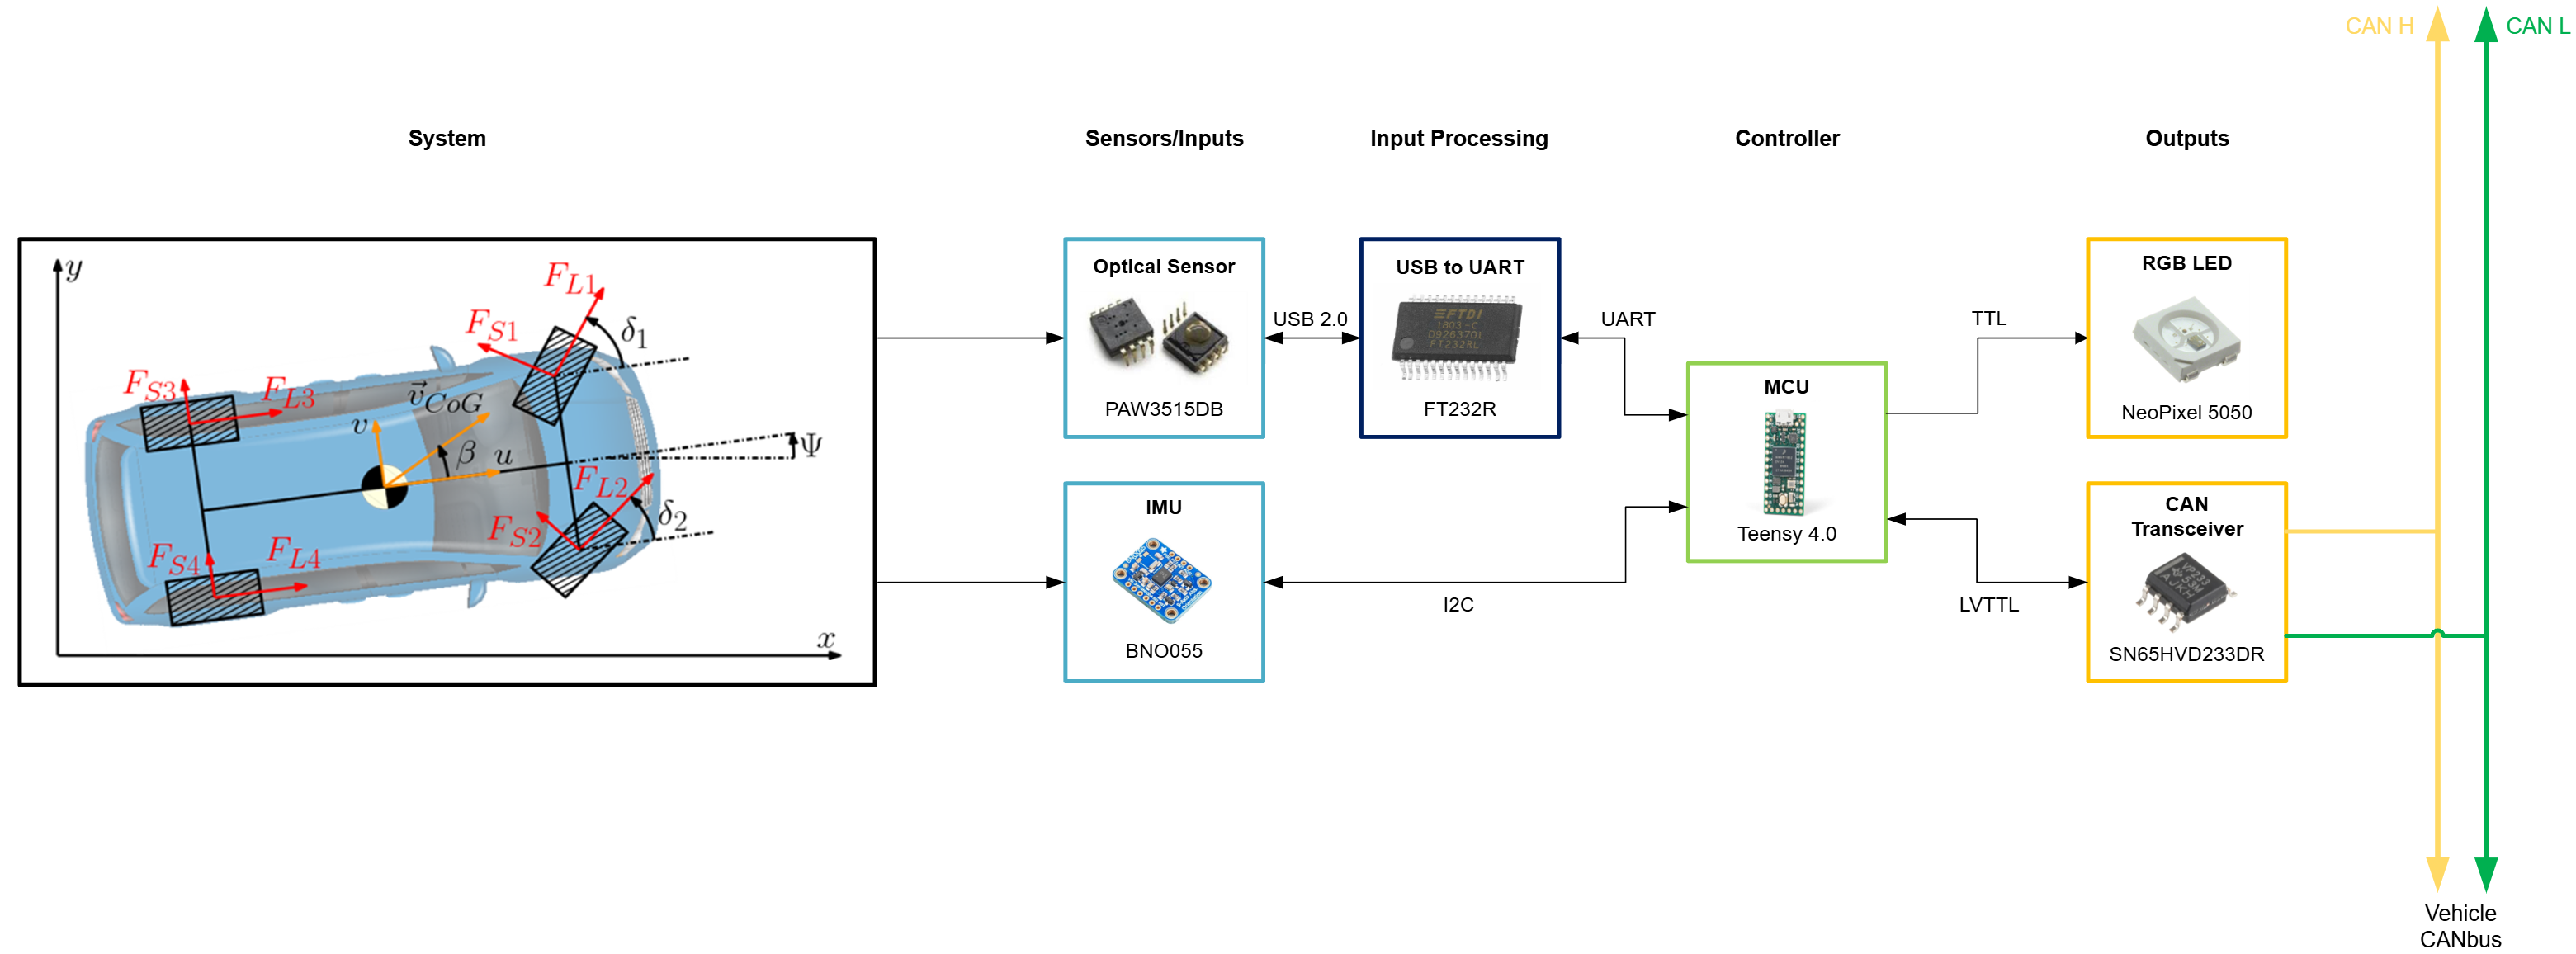
\includegraphics[width=1\textwidth]{resources/Screenshot 2025-04-27 181552.png}

            \vspace{0.5cm}

            \textbf{Figure 7: Hardware Diagram}
            \label{hd}
        
        \end{center}

        % words and text

        % \begin{center}
        %     \vspace{0.5cm}

        %     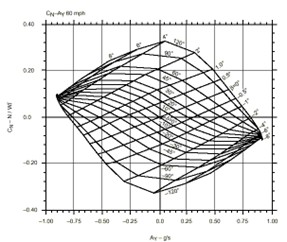
\includegraphics[width=0.5\textwidth]{resources/tn_MMM807.jpg}

        %     \vspace{0.5cm}

        %     \textbf{Figure 7: Intended Application}
        %     \label{ia}
        
        % \end{center}
        
        \subsection{Microcontroller (Teensy 4.0)}

            The Microcontroller Development Board selected for this project is the Teensy 4.0, powered by NXP’s i.MX RT1062 microcontroller. This device 
            features an Arm Cortex‑M7 core running at 600 MHz, making it one of the fastest Cortex-M-based MCUs available. The core is accompanied by a 
            hardware floating‑point unit (FPU) and digital signal processing (DSP) extensions, making it ideally suited for real-time control, signal 
            processing, and multimedia applications. Additionally, it leverages a dual-issue pipeline, meaning it can execute two instructions in one 
            clock cycle, branch prediction, dual 32 KB caches, and tightly-coupled memory for single-cycle access to time-critical data and instructions 
            \autocite{PJRC}. 

            The Teensy 4.0 is equipped with 1984 KB of Flash, 1024 KB of RAM (512 KB tightly coupled), and 1 KB of emulated EEPROM. It exposes 40 digital 
            I/O pins, 14 analog inputs with up to 12-bit resolution, and 31 PWM-capable pins. Standard communication interfaces such as I²C, UART, and SPI 
            are supported, along with more advanced options like USB 2.0 OTG (480 Mbps host/device), dual CAN-FD controllers, and a 10/100 Ethernet MAC. It 
            also includes essential embedded timers such as the SysTick, real-time clock (RTC), and a watchdog timer, providing a highly flexible platform 
            for a wide range of embedded system designs \autocite{PJRC}.

            In terms of core processing power, the Teensy 4.0 significantly outperforms comparable microcontroller boards. It dwarfs the 240 MHz dual core 
            Xtensa LX6 of ESP32 modules, far exceeds the 72 MHz Cortex-M3 of the STM32 Blue Pill and substantially outpaces the 64 MHz Cortex-M0+ or Cortex-M4 
            cores found in boards like the Arduino Nano 33 IoT and Nano 33 BLE Sense. For compute-heavy tasks such as slip-angle calculations, its tightly 
            coupled RAM and NVIC interrupt controller allow real-time deadlines to be met without the cache misses or RTOS jitter that can plague multicore 
            ESP32s or lower-clocked STM32/AVR alternatives. 

            The peripheral set also makes the Teensy a superior choice for our slip-angle application. While the Arduino Nano lacks any USB host capability or 
            CAN support, and the STM32F103 only supports Full-Speed USB and legacy CAN 2.0, the Teensy 4.0 offers all the required communication interfaces 
            needed for this project. It can simultaneously log high-rate sensor data via a USB-to-UART bridge, like the FT232R chip, and transmit slip-angle 
            results across the vehicle’s CAN-FD bus. For analog tasks, Teensy supplies 14 ADC channels, compared to 8 on the Nano and 10 on the STM32F103, 
            and 31 PWM outputs for potential actuator control, which again outpaces what similar boards can deliver.

            Programming the teensy can be done through a variety of mediums including the Arduino IDE (via the Teensyduino plug‑in) or in PlatformIO, providing 
            a rapid, user‑friendly workflow. For in‑depth development and troubleshooting, the i.MX RT1062 implements ARM CoreSight with SWD/JTAG access. 
            Additionally, its Nested Vectored Interrupt Controller (NVIC) supports deterministic and priority-based interrupt handling, allowing for example, 
            slip angle computations to interrupt lower priority routines with negligible overhead, while optional JTAG pads enable real‑time trace capture and 
            hardware breakpoints for advanced optimization. Unlike the Arduino Nano’s limited bootloader or the ESP32’s manual upload process, the Teensy’s 
            dedicated loader chip enables fast, reliable flashing without sacrificing any program Flash memory.

            Together, these capabilities make the Teensy 4.0, and by extension the i.MX RT1062, an exceptionally powerful yet compact platform for embedded 
            systems development, offering significant advantages over other microcontroller solutions available on the market.

        \subsection{Optical Sensor (PAW3515DB)}
            
            The PAW3515DB is a compact, single-chip optical motion sensor originally designed for USB mice. It features a CMOS image sensor and an onboard digital 
            signal processor capable of detecting precise two-dimensional surface motion at speeds up to 30 inches per second, resolutions up to 1600 counts per inch, 
            and a frame rate of 3300 frames per second. Its ability to continuously track relative motion across textured surfaces makes it a strong candidate for 
            slip angle detection applications. In this context, the sensor is mounted beneath a vehicle, facing downward toward the road surface. By optically 
            tracking the motion of the ground beneath the contact patch of the tire through a LED, the PAW3515DB outputs lateral and longitudinal movement as 
            $\Delta$X and $\Delta$Y displacement vectors. When these vectors are compared against the vehicle's heading, the angular difference reveals the slip angle. 
            This provides a direct, ground-referenced method for capturing real-world tire behavior during dynamic driving conditions.

            The PAW3515DB was selected for three key reasons. First, it is extremely cost-effective, offering a viable alternative to professional grade slip 
            angle sensors, which can be prohibitively expensive. Second, it is a self-contained, integrated optical flow sensor, with all the processing handled 
            internally, eliminating the need for developing a custom optical system from scratch. Additionally, the PAW3515DB is far easier to integrate into our 
            design given that it's a DIP8 IC. Lastly, the optical flow-based motion estimation method, which forms the core sensing principle of this chip, is 
            fundamentally the same as that is used in many high-end slip angle sensors, with the PAW3515DB achieving similar functionality at a fraction of the cost.

            While high end mouse sensors like the PMW3360 offer higher CPI values, they are optimized for smooth indoor surfaces and can become unreliable on rough, 
            high-contrast textures like asphalt. Sensors like the ADNS-9800, originally designed for laser-based optical mice, perform poorly outdoors due to their 
            sensitivity to ambient infrared light and are not well-suited for direct ground tracking under varying lighting conditions. In contrast, the PAW3515DB 
            strikes an excellent balance between frame rate, surface adaptability, and robustness.

            \subsubsection{USB to UART (FT232R)}
                
                The FT232R, developed by FTDI, is a versatile and widely adopted USB to UART interface chip that enables seamless communication between USB-equipped host 
                devices and UART-based peripherals. In this system, it plays a critical role by allowing the PAW3515DB optical motion sensor, which outputs serial data 
                over UART, to interface with the Teensy 4.0 microcontroller through a USB connection. The FT232R handles all low-level USB protocol operations internally, 
                presenting a standard UART interface to the Teensy while appearing as a virtual COM port to the operating system \autocite{FTDIChip}.

                The FT232R features a full-speed USB 2.0 interface (12 Mbps), integrated clock generation (eliminating the need for an external crystal), on-chip EEPROM for 
                configuration, and flexible handshaking options such as RTS/CTS and DTR/DSR. It supports data rates up to 3 Mbps, far exceeding the baud rate requirements 
                of the PAW3515DB, ensuring that high-frame-rate displacement data can be transmitted with negligible latency or data loss. Furthermore, the chip includes 
                a programmable CBUS interface, which can be used for extra I/O functions like driving LEDs or enabling power management \autocite{FTDIChip}.

                Compared to alternative USB-UART solutions such as the CH340G or CP2102, the FT232R provides superior driver support across Windows, Linux, and macOS platforms, 
                along with lower latency USB-UART bridging and robust error recovery mechanisms. Its well-documented API (D2XX) and long-standing industry reliability make 
                it a natural choice for critical embedded applications where communication stability is paramount. By integrating the FT232R, the system gains a robust, 
                high-speed, and low-overhead method of relaying optical sensor data to the Teensy 4.0, enabling accurate real-time ground motion tracking essential for 
                slip angle calculations.

        \subsection{Inertial Measurement Unit (BNO055)}

            The BNO055 is a compact, 9-axis inertial measurement unit developed by Bosch that integrates a 3-axis 16-bit gyroscope, 3-axis 14-bit accelerometer, and 
            a 3-axis high-resolution magnetometer, along with a built-in ARM Cortex-M0+ processor for onboard sensor fusion. Unlike conventional IMUs that stream raw 
            X-, Y-, and Z-axis data, the BNO055 internally runs Bosch’s fusion algorithm, performing quaternion mathematics, bias correction, and magnetometer calibration 
            directly on-chip. It outputs fully fused orientation data including quaternions, Euler angles (roll, pitch, yaw), rotation vectors, linear acceleration, 
            gravity vectors, and absolute heading at up to 100 Hz via standard I²C or high-speed UART \autocite{BOSCH}.

            The sensor supports multiple power modes (normal, low power, suspend) and programmable ranges from ±2g to ±16g for acceleration and ±125°/s to ±2000°/s 
            for rotation, with built-in temperature compensation that keeps yaw drift to just a few degrees per minute. Its ability to deliver drift-compensated orientation 
            without external processing makes it ideal for vehicle heading estimation and slip-angle detection applications \autocite{BOSCH}.

            Compared to popular raw IMUs like the MPU-6050, MPU-9250, ICM-20948, or the LSM9DS1, the BNO055 greatly reduces host MCU burden by offloading the sensor fusion 
            computations internally, freeing CPU time for higher level control and telemetry tasks. Its self-calibration stores offsets automatically into non-volatile 
            memory, avoiding the complex manual tuning that raw IMUs typically require. Breakout boards from Adafruit \& SparkFun operate seamlessly at 3.3V logic and 
            integrate easily with the Teensy’s workflow. This makes the BNO055 an excellent choice for this system.

        \subsection{RGB LED (NeoPixel 5050)}

            Here an RGB can be utilized as a status indicator for the device. When the system is powered on and functioning normally, the LED displays green, signaling 
            active and healthy operation. If an error is detected during runtime, such as a communication failure with the PAW3515DB or BNO055, or an internal sensor 
            malfunction, the LED switches to red to immediately alert the user to an error condition. When the device is in an idle or powered off state, the LED remains 
            off, conserving power and clearly indicating inactivity. This real-time visual feedback allows for simple and immediate system diagnostics without requiring 
            an external display or serial monitor.

        \subsection{CAN Transceiver (SN65HVD233DR)}

            The SN65HVD233DR is a high-speed CAN transceiver developed by Texas Instruments, designed to support communication rates up to 1 Mbps and fully compatible 
            with ISO 11898-2 and ISO 11898-5 standards. As a critical bridge between the microcontroller's CAN controller and the physical vehicle bus, the transceiver 
            translates the Teensy 4.0’s differential CAN signals into robust, noise-resistant electrical levels suitable for in-vehicle networking. Operating at a wide 
            supply range from 3.0V to 3.6V and featuring a true 3.3V I/O interface, it is ideal for integration with the Teensy 4.0’s 3.3V logic. The SN65HVD233DR also 
            supports low-power standby modes and has integrated protection features, including thermal shutdown, short-circuit protection, and transient protection, 
            enhancing system reliability under harsh automotive conditions \autocite{TI}.

            One of the standout features of the SN65HVD233DR is its silent mode capability, allowing the device to listen passively on the CAN bus without actively 
            driving the bus lines. This is particularly useful during initial testing, diagnostic operations, or when implementing multi-node systems where bus arbitration 
            must be carefully managed. Additionally, its robust common-mode range of –2V to +7V ensures reliable operation even in electrically noisy environments such 
            as electric vehicles. In the context of this project, the transceiver enables the Teensy 4.0 to transmit slip angle and motion data directly onto the vehicle’s 
            high-speed CANbus with minimal latency, providing an industry-standard interface for logging, diagnostics, or active control applications.

    \section{Software Design}

        \begin{center}
            \vspace{0.5cm}

            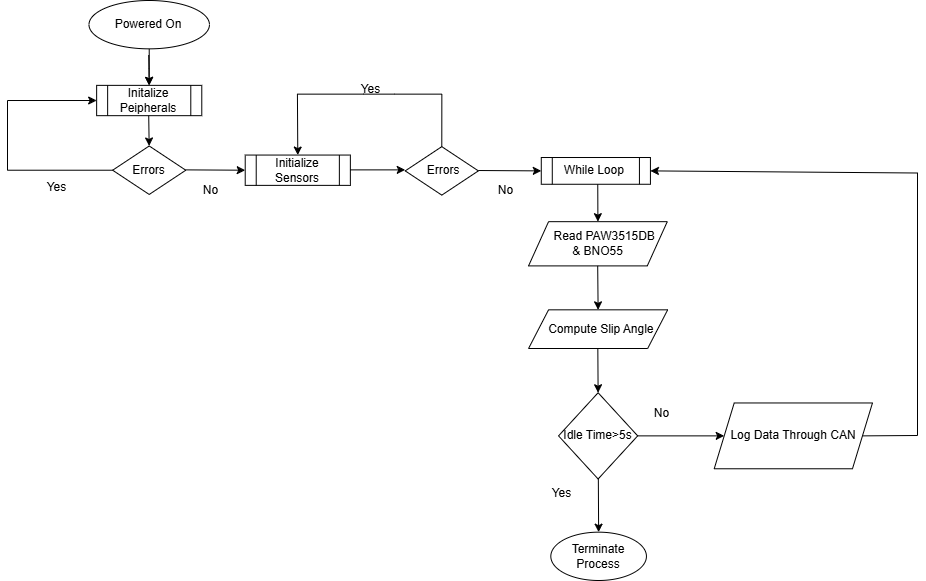
\includegraphics[width=1\textwidth]{resources/softwarediagram.png}

            \vspace{0.5cm}

            \textbf{Figure 8: High-Level Software Design}
            \label{sd}
        
        \end{center}

        % On powering up the system, the firmware first configures the microcontroller’s peripheral interfaces which includes the CAN host, GPIO inputs for 
        % the PAW3515DB, I²C for the BNO055, the CAN transceiver, and the RGB status LED, then performs an error check. Any failure routes execution back to an 
        % error‑recovery loop until the fault is cleared. Once the interfaces pass, the program configures the sensors, loading their operating modes and verifying 
        % that both the optical‑flow unit and the IMU return valid data. Next, the program enters a continuous while‑loop in which the microcontroller repeatedly 
        % acquires ground motion vectors ($\Delta$X, $\Delta$Y) from the PAW3515DB and yaw orientation data from the BNO055, and then proceeds to compute the instantaneous slip 
        % angle by subtracting vehicle heading from the optical motion direction, and broadcasts the result onto the vehicle’s CAN bus for telemetry. An inactivity 
        % timer monitors motion, where if no meaningful movement is detected for five seconds, the system exits the loop and executes a clean shutdown sequence. 
        % Throughout, any peripheral or sensor error immediately diverts execution back to the recovery branch, ensuring robust fault handling without compromising 
        % real‑time operation.

        \subsection{Peripheral Initialization Block}

            Upon powering up the system, the firmware first configures all essential microcontroller peripherals necessary for operation. This includes initializing 
            the CAN interface for real-time telemetry transmission, configuring GPIO inputs required to interface with the PAW3515DB optical flow sensor, setting up 
            I²C communication to the BNO055 IMU, activating the CAN transceiver, and enabling the RGB status LED used for visual system monitoring. The CAN controller 
            is configured for standard and extended frame operation, and the UART/I²C peripherals are assigned appropriate baud rates and interrupt priorities. An error 
            check is performed after each peripheral setup to ensure correct operation. If any fault is detected, such as a peripheral not responding, the system routes 
            execution back to an initialization recovery loop that retries peripheral setup. This guarantees that no subsequent steps are attempted unless a stable baseline 
            hardware configuration is achieved.

        \subsection{Sensor Initialization Block}

            Following successful peripheral configuration, the firmware proceeds to initialize the key sensors. The PAW3515DB is placed into its motion-tracking mode, 
            while the BNO055 is configured to output fused Euler angles via I²C, minimizing CPU post-processing. Sensor specific interrupts, such as motion triggered events, 
            are configured but masked until system readiness is confirmed. The system verifies that valid sensor data is being returned from both units through a validation 
            check. Any failed initialization, incorrect register configuration, or communication timeout returns control to the recovery loop for retry. This layered sensor 
            validation ensures both ground motion and vehicle heading data are available before entering active system operation.

        \subsection{Main Operational Loop}

            Once peripherals and sensors have been successfully initialized, the firmware enters the main real-time operational loop. Within this loop, the microcontroller performs 
            the following tasks at a fixed sampling rate:

            \subsubsection{Sensor Acquisition}

                Periodically reads $\Delta$X and $\Delta$Y motion vectors from the PAW3515DB, and yaw orientation angles from the BNO055. 

            \subsubsection{Slip Angle Computation}

                Computes the instantaneous slip angle in real time by applying an arctangent (atan2) function to the $\Delta$Y/$\Delta$X motion vector and subtracting the 
                fused heading from the BNO055. Minor signal processing via low-pass filtering may be optionally applied by the IMU to stabilize computed values.

            \subsubsection{Data Transmission}

                The computed slip angle and supporting telemetry are packaged into CAN frames and transmitted over the CAN bus at regular intervals, using non-blocking 
                transmission queues to ensure no packet loss during high-load conditions.

            \subsubsection{Real-Time System Management}

                The system utilizes the microcontroller’s Nested Vectored Interrupt Controller to prioritize critical events, such as sensor data availability and CAN transmission, 
                ensuring deterministic, low-latency real-time performance.

            \subsubsection{Idle Detection and Power Management}

                An inactivity timer monitors system motion. if no significant displacement is detected for more than five seconds, the system exits the loop and executes a 
                clean shutdown sequence, optionally placing peripherals into low-power states and disabling telemetry.
    
    \section{Contributions}

        The project was evenly divided between Nathan Quadras and Kosta Sergakis. Kosta proposed and refined the project idea and was responsible for the Overview \& Motivation, 
        Hardware Interfacing, system-level communication requirements, and final document formatting. Nathan handled the descriptions of system components, including the 
        Microcontroller, IMU, Optical Sensor, and LED, as well as the development of the Software Design and Architecture.
    
    % % % % % % % % %
    % Bibliography  %
    % % % % % % % % %

    % \addcontentsline{toc}{section}{Works Cited}
    % \printbibliography
    \newpage
    \phantomsection % Create a phantom section to get the correct page number in the ToC
    \addcontentsline{toc}{section}{Works Cited}
    \printbibliography[title=Works Cited]

    % \bibliographystyle{plainnat}
    % \bibliography{sources}

\end{document}